\subsection{Analisi}
Periodo: dal 2019-11-15 al 2020-01-20\\
Inizia con la formazione del gruppo e finisce con la data di consegna per la Revisione dei Requisiti.\\
In questa fase viene definito il gruppo, la normazione (\glo{way of working}) e la garanzia di qualità che si vuole fornire, oltre alla definizione dei requisiti del capitolato che viene scelto.

\subsubsection{Periodo 1}
Dal 2019-11-15 al 2019-11-29\\
In questo periodo, che parte dalla formazione del gruppo e termina con la scelta del capitolato C5 \NomeProgetto{}, il gruppo intende affrontare le seguenti tematiche al fine di porre le basi per il lavoro che va affrontato:
\begin{itemize}
	\item \textbf{Discussione capitolati}: Ogni membro del gruppo studia individualmente e in seguito discute con gli altri membri durante gli incontri tutti i capitolati proposti, ponendo le basi per la stesura del documento \SdF{} e indirizzando la scelta del capitolato;
	\item \textbf{Assegnazione e studio dei ruoli di progetto}: Ad ogni membro del gruppo viene assegnato il ruolo principale da ricoprire nella fase di Analisi;
	\item \textbf{Definizione degli strumenti}: Vengono discusse e definite le tecnologie da usare per affrontare la fase di Analisi;
	\item \textbf{Pianificazione milestone fase di Analisi}: Vengono discusse e fissate delle \glo{milestone} intermedie da rispettare per completare la fase di Analisi entro le scadenze imposteci.
\end{itemize}

\subsubsection{Periodo 2} 
Dal 2019-11-30 al 2019-12-31\\
Questo periodo inizia con la scelta definitiva del capitolato C5 \NomeProgetto{}.\\
Dopo la scelta, vanno focalizzate le risorse del gruppo nei seguenti punti:
\begin{itemize}
	\item \textbf{Normazione}: Vengono definite le regole per la stesura dei documenti e per l'utilizzo delle tecnologie identificate in precedenza;
	\item \textbf{Approfondimento capitolati}: Vengono ulteriormente discussi tutti i capitolati in modo da terminare lo \SdF{} e focalizzare l'attenzione sull'analisi del capitolato scelto in modo da predisporre le basi per l'\AdR{};
	\item \textbf{Prima definizione dei casi d'uso}: Attività dove vengono identificati ed analizzati i requisiti del capitolato, cercando di comprendere come il sistema debba essere realizzato;
	\item \textbf{Determinazione standard di qualità}: Vengono definite le strategie per garantire la qualità di \glo{processo} e la qualità di prodotto;
	\item \textbf{Verifica}: \glo{Verifica} dell'andamento del gruppo in relazione alle tempistiche e allo svolgimento dei compiti assegnati.
\end{itemize}

\subsubsection{Periodo 3}
Dal 2020-01-01 al 2020-01-14\\
Questo periodo si estende fino alla data ultima di consegna per affrontare la Revisione dei Requisiti a cui il gruppo ha deciso di partecipare.
\begin{itemize}
	\item \textbf{Normazione}: Ulteriori approfondimenti alle regole per la stesura dei documenti e per l'utilizzo delle tecnologie;
	\item \textbf{Approfondimento delle tecnologie}: Vengono ampliate le conoscenze sulle tecnologie richieste dal capitolato per essere svolto;
	\item \textbf{\AdR{}}: Studio dei requisiti e raffinamento dei casi d'uso;
	\item \textbf{Pianificazione delle attività}: Pianificazione del lavoro da svolgere nelle fasi successive a quella di Analisi;
	\item \textbf{Verifica}: \glo{Verifica} dell'andamento del gruppo in relazione alle tempistiche e allo svolgimento dei compiti assegnati.
\end{itemize}

\subsubsection{Periodo 4} 
Dal 2020-01-15 al 2020-01-20\\
In questo periodo, che ha inizio con la consegna della documentazione prodotta per la Revisione dei Requisiti alla presentazione pubblica della proposta, il gruppo consolida il lavoro svolto in vista delle successive fasi e della discussione per la quale serve una presentazione:
\begin{itemize}
	\item \textbf{Consolidamento}: Ogni membro del gruppo si prende del tempo per ripassare tutto il lavoro svolto e per studiare il necessario per affrontare al meglio le fasi successive;
	\item \textbf{Preparazione per la Revisione dei Requisiti}: Il gruppo produce il materiale necessario da esporre alla presentazione pubblica della propria proposta.
\end{itemize}

%PAGINA ORIZZONTALE
\newpage
\paperwidth=\pdfpageheight
\paperheight=\pdfpagewidth
\pdfpageheight=\paperheight
\pdfpagewidth=\paperwidth
\headwidth=\textheight

\begingroup 
\vsize=\textwidth
\hsize=\textheight

\subsubsection{Diagramma di Gantt delle attività della fase di Analisi}
\pagestyle{empty}
\begin{figure}[h]
	\centering	
	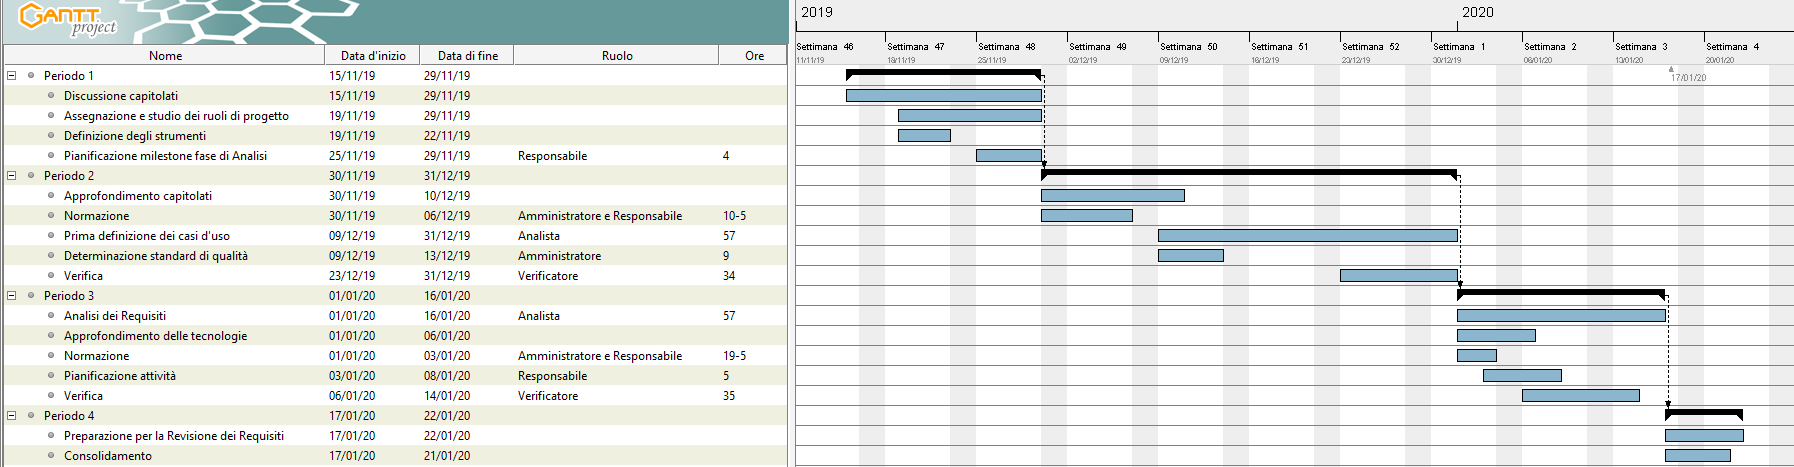
\includegraphics[height = 9cm, width = 24.5cm]{Sezioni/DiagrammiGantt/Analisi.png}
	\caption{Diagramma di Gantt delle attività della fase di Analisi}
\end{figure}

\textwidth=\hsize
\textheight=\vsize

\endgroup
\newpage
\paperwidth=\pdfpageheight
\paperheight=\pdfpagewidth
\pdfpageheight=\paperheight
\pdfpagewidth=\paperwidth
\headwidth=\textwidth